\documentclass[english,serif,mathserif]{beamer}
\usetheme[formal,deutsch]{s3it}

\usepackage[T1]{fontenc}
\usepackage[latin9]{inputenc}
\usepackage{babel}

\begin{document}

%% Optional Argument in [Brackets]: Short Title for Footline
\title[Short Title]{Cinder}
\subtitle{Or: Openstack's Block Storage Service}

\author{Tyanko Aleksiev \texttt{<tyanko.aleksiev@s3it.uzh.ch>}}

\date{\today}

\maketitle

\begin{frame}{Cinder's role inside OpenStack}

Cinder is a service used to provide Virtualized Block Storage Devices to the 
end users of OpenStack without requiring them to have any knowledge of where 
that storage is actually deployed or on what type of device. 

\end{frame}

\begin{frame}{Cinder's components: \textbf{cinder-api}}

The role of cinder-api is to accept and manage API calls to:

\begin{itemize}
\item create, delete, list and show volumes,
\item create, delete, list and show snapshots,
\item attach and detach volumes (called by nova).
\end{itemize}

\end{frame}

\begin{frame}{Cinder's components \textbf{cinder-volume}}

cinder-volume is:
\begin{itemize}
\item handling all the requests coming from cinder-api, 
\item is keeping the Block Storage Database up to date,
\item is interacting with other processes (like cinder-scheduler) through the message queue,
\item is interacting directly with variuos types of storage back-ends.
\end{itemize}

Multiple cinder-volumes instances can be run using different configuration files and
back-ends to allow scalabilty but also one cinder-volume can be manage multiple back-ends.

\end{frame}

\begin{frame}{Cinder's components \textbf{cinder-scheduler}}

cinder-scheduler's main role is choosint the best back-end to use for placing the new volume. 
It interacts with cinder-volume through the message queue and the Block Storage Database 
and can be decoupled from the host running cinder-{api,volume}. Different filters are available 
as plug-ins.

\end{frame}

\begin{frame}{Cinder's components: \textbf{message queue}}

The message queue is used for communication between the Cinder's components.  

\end{frame}

\begin{frame}{Cinder: components interaction 1/2}

\centerline{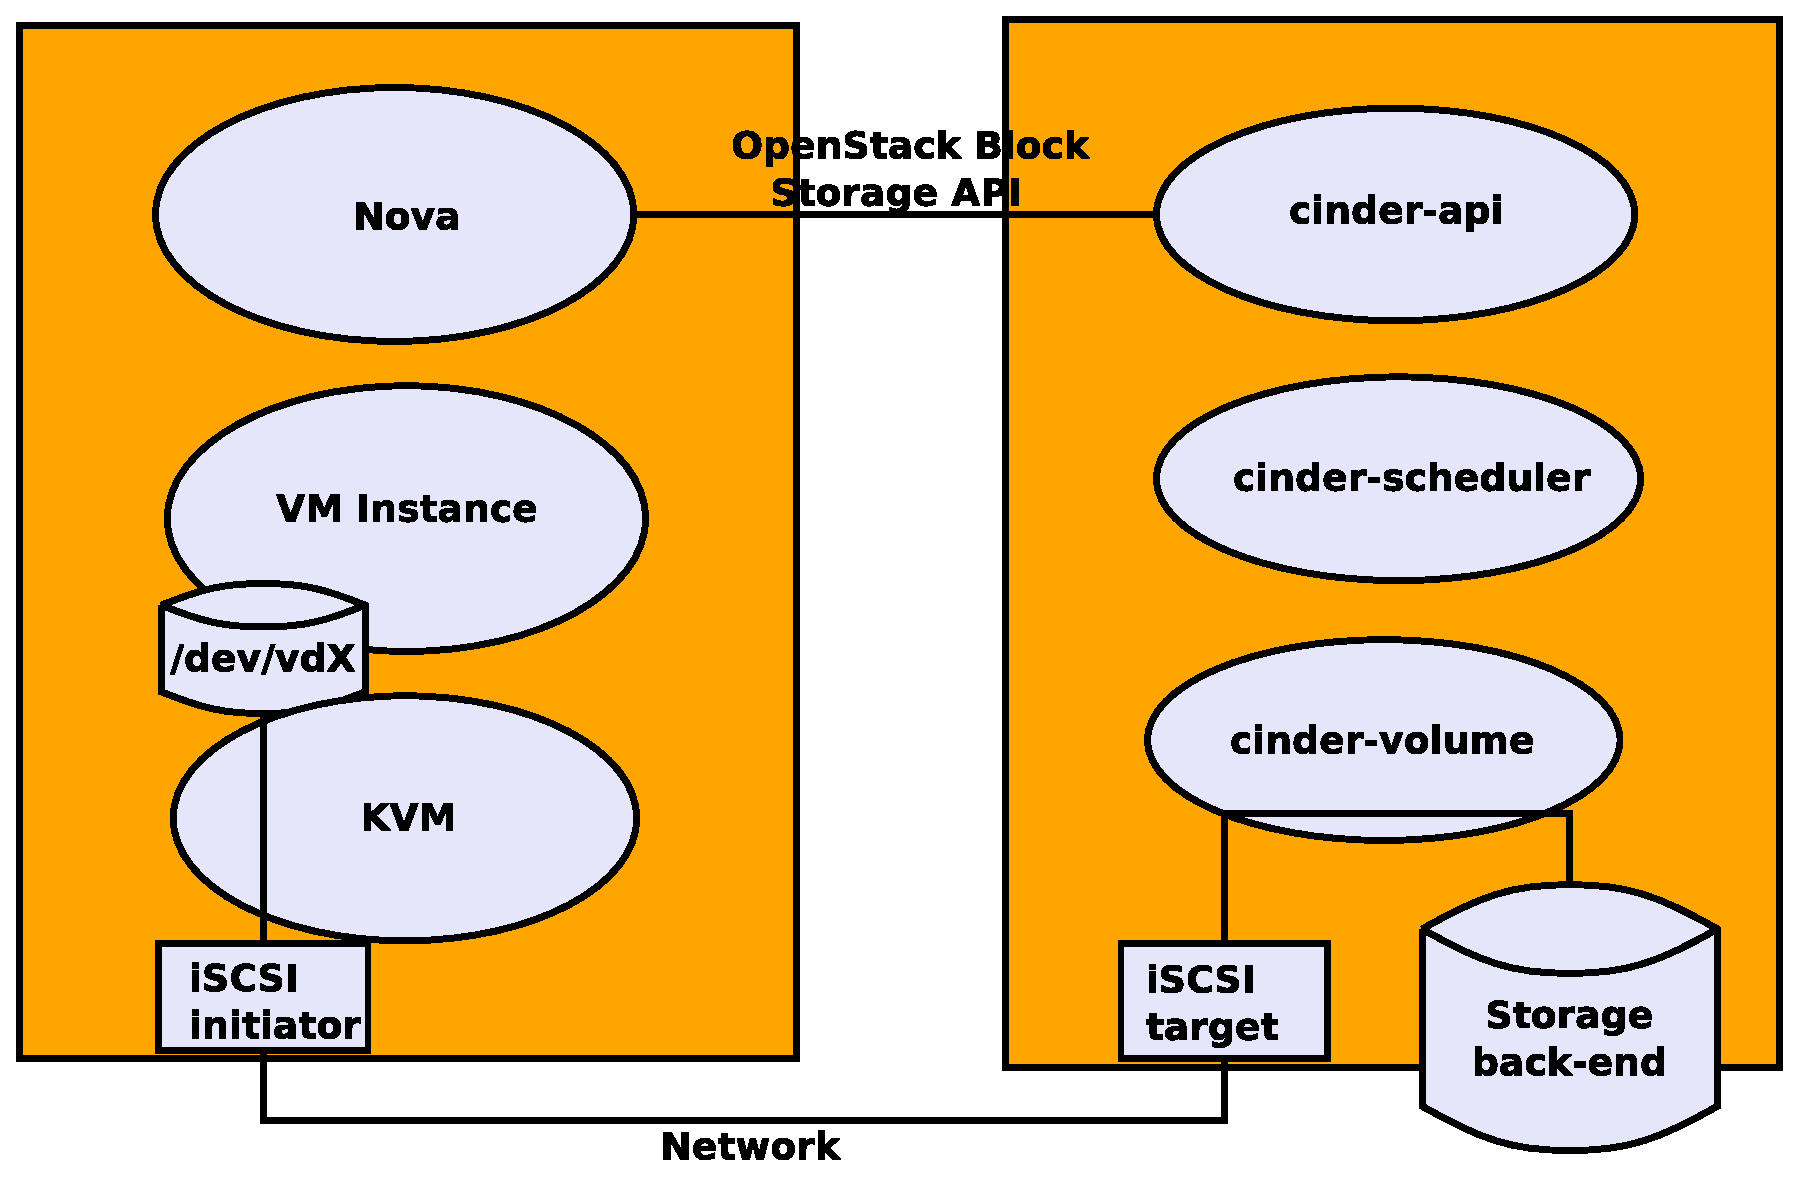
\includegraphics[scale=0.30]{cinder.eps}}

\end{frame}

\begin{frame}{Cinder: components interaction 2/2}

Interaction example:

\begin{itemize}
\item nova calls cinder-api via API providing connection information (hostname, iSCSI initiator name, etc),
\item cinder-api passes the message to cinder-volume,
\item cinder-volumes calles the storage volume driver or uses the queue to ask cinder-scheduler for a good candidate,
\item the storage volume driver does everything to allow the connection (eg. give access),
\item the storage volume driver returns connection information to nova,
\item nova creates then the connections using the given parameteres,
\item nova passes the volume device/file to the hypervisor.  
\end{itemize}

\end{frame}

\begin{frame}{Notes and Remarks}

\begin{itemize}
\item Logs directory is: \texttt{/var/log/cinder}
\item Files you are going to edit often:
      \begin{itemize}
        \item cinder-api conf. file is: \texttt{/etc/cinder/cinder-api.conf}
        \item cinder-volume conf. file is: \texttt{/etc/cinder/cinder-volume.conf}
      \end{itemize}
\item We will see everything in more detail during the tutorial.
\end{itemize}

\end{frame}

\begin{frame}{Useful Links}

\begin{itemize}
\item \href{http://docs.openstack.org/icehouse/install-guide/install/apt/content/ch\_cinder.html}{Configure Cinder}
\item \href{https://wiki.openstack.org/wiki/Cinder}{Cinder Project Documentation}
\end{itemize}

\end{frame}



\end{document}

%%% Local Variables:
%%% mode: latex
%%% TeX-master: t
%%% End:
